% !TEX root = ../thesis.tex

\chapter{Stand der Forschung}\label{chap:forschung}

Dieses Kapitel betrachtet die Schwarmzustände, welche in Fischschwärmen nachgewiesen wurden.
Daraufhin folgt die Definition der Modelle, mit deren Hilfe die Zustände abgebildet werden sollen.

\section{Zustände von Schwärmen}\label{sec:Zustaende}

Viele Schwärme zeigen koordiniertes Verhalten, das durch das Zusammenspiel der einzelnen Individuen zustande kommt. Dies lässt sich auf das autonome Verhalten der einzelnen Agenten zurückführen. Schwärme, dessen Agenten den Regel von Reynolds (vgl. \ref{sec:Boids}) folgen zeigen drei unterschiedliche Zustände. Diese werden in dem Papter ''Collective States, Multistability and Transitional Behavior in Schooling Fish'' als \textit{swarm}, \textit{polarized} und \textit{milling} bezeichnet \cite{Tunstrm2013CollectiveSM} .

\begin{figure}[h]
\centering

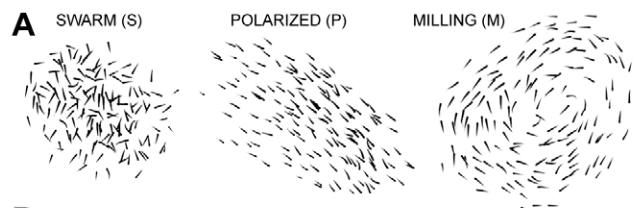
\includegraphics[width=0.7\textwidth]{figures/Forschung/states.png} 

\caption{Zustände von Fischschwärmen \label{fig:Zustaende}, entnommen aus \citep{Tunstrm2013CollectiveSM}}
\end{figure}

\textit{Swarm} bezeichnet globale und lokale Unstrukturiertheit. Hierbei ist die Ausrichtung der Agenten scheinbar zufällig. Dies ist in Abbildung \ref{fig:Zustaende} links zu sehen. Hierbei findet zum größten Teil keine Bewegung des Schwarms als Ganzes statt.

\textit{Polarized} wird der Zustand, der im mittleren Bild zu sehen ist, genannt.
In diesem Zustand sind die Agenten gleich ausgerichtet. Der Schwarm bewegt sich dadurch als Ganzes in eine Richtung.

\textit{Milling} ist der Zustand, der im rechten Bild zusehen ist. Die Agenten kreisen um einen Punkt. Hier findet ebenfalls eine Bewegung des Schwarms statt. Der Schwarm bewegt sich hier lokal an einer Stelle.


Ist der Schwarm im \textit{Polarized} Zustand, so ist die Richtung der Agenten größtenteils gleich. Mittelt man über die normierten Richtungsvektoren $u_i$ der Agenten, gibt die Länge des hieraus resultierenden Vektors Aufschluss auf das Vorhandenseins dieses Zustands.

Der Zustand \textit{Milling} kann auf ähnliche Weise ermittelt werden. Hierzu wird der Vektor $r_i$ berechnet, der von Agent $i$ in Richtung Mittelpunkt des Schwarms zeigt. Vergleicht man nun die Vektoren $r_i$ und $u_i$ so kann festgestellt werden, ob der Schwarm rotiert.
Dies ist der Fall, wenn $r_i$ und $u_i$ im rechten Winkel zueinanderstehen.


\begin{subequations}
\begin{align}
O_p &= \frac{1}{N} \left\vert \sum_{i=1}^{N}u_i\right\vert \label{eq:Op} \\
O_r &= \frac{1}{N} \left\vert \sum_{i=1}^{N}u_i \times r_i\right\vert \label{eq:Or}
\end{align}
\end{subequations}

In obenstehender Gleichung ist die Berechnungsvorschrift für den \textit{Polarized}-Zustand (\ref{eq:Op}) und dem \textit{Milling}-zustand (\ref{eq:Or}) zu sehen.



Eine wichtige Erkenntnis ist, dass die Zustände koexistieren können. 
Weiter werden die Zustände Anhand der Werte von $O_p$ und $O_r$ definiert.
\begin{itemize}
	\item Der polarisierte Zustand ist erreicht wenn: $O_p > 0.65$ und $O_r < 0.35$ 
	\item Der Rotationszustand ist erreicht wenn: $O_r > 0.65$ und $O_p < 0.35$ 
	\item Der Schwarmzustand ist erreicht wenn: $O_p < 0.35$ und $O_r < 0.35$ 
\end{itemize}

Diese Schranken werden im weiteren Verlauf als Maßgebend für das Vorhandensein eines Zustandes sein.

\section{Modelle}\label{sec:Modelle}

Die Modellbeschreibung, wie sie in Abschnitt \ref{sec:Boids} beschrieben wurden, definieren noch kein explizites Modell.
In diesem Teil des Kapitels werden zwei Modelle vorgestellt. Auf das erste Modell trifft man des öfteren in der gängigen Literatur. Teilweise auch in abgewandelter Form. Die hier gewählte Form wird verwendet, da es in Zusammenhang mit den drei vorgestellten Zuständen steht. Das zweite Modell ist eines, welches aus eigenen Überlegungen entstand. Hierbei wird eine eigene Interpretation der Schwarmzustände in Einklang mit einem Modell gebracht.

\subsection{Metrisches Modell}\label{sec:metrischesModell}
Wie bereits angesprochen, fundieren die agentenbasierten Modelle auf den drei Grundannahmen des Abstandhaltens, Angleichens und Zusammenbleibens. Der Versuch, die typischen Eigenschaften eines Schwarms zu simulieren, wurde von in dem Paper ''Collective memory and spatial sorting in animal groups'' präsentiert \cite{Couzin2002CollectiveMA}.
Hierbei wird auf ein Modell gesetzt, das den metrischen Ansatz verfolgt.

\begin{figure}[H]
\centering

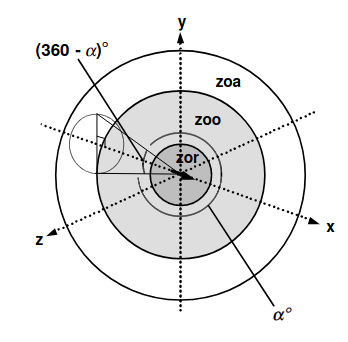
\includegraphics[width=0.6\textwidth]{figures/Forschung/metrisch.png} 

\caption{Zonen im metrischen Modell eines Agenten nach \cite{Couzin2002CollectiveMA}, Abbildung entnommen aus selbigen Paper \label{fig:Metrisch_couzin}}
\end{figure}

Der Wahrnehmungsbereich eines Agenten besteht aus drei Zonen. Die innerste Zone des Models ist die Abstandhaltenzone. In Abbildung \ref{fig:Metrisch_couzin} \textbf{zor} (zone of repulsion) bezeichnet. Diese Zone hat die höchste Priorität. Befinden sich Agenten in dieser Zone, so haben andere Zonen keinen Einfluss auf das Verhalten des Agenten. Dies ist laut \citet{inbook} ein häufig beobachtetes Phänomen im Tierreich. Die nachfolgende Gleichung legt das Verhalten des Agenten für diesen Zonenbereich dar.

\begin{subequations}
\begin{align}
d_r(t+\tau) &= - \sum_{j\neq i}^{n_r} \frac{r_{ij}(t)}{|r_{ij}(t)|} \label{eq:rp} 
\end{align}
\end{subequations}

Finden sich Agenten in dieser Zone, so bewegt sich der Agent in Richtung $d_i(t+\tau) = d_r(t+\tau)$.
Der Vektor $r_{ij}(t)$ ist der Vektor, der zum Nachbaragenten $j$ zeigt. Gleichung \ref{eq:rp} beschreibt hier das sich Entfernen des Agenten $i$ von dem lokalen Massezentrum welches durch die Agenten $j$ entsteht. Für den Fall, dass $n_r = 0$ ist, kommen die Zonen \textbf{zoo} (zone of orientation) und \textbf{zoa} (zone of attraction) zu tragen. 

Der Agent $i$ gleicht seine Orientierung den Orientierungen der Agenten $j$, die sich in der \textbf{zoo} befinden, an.
Dies lässt sich durch folgende Vorschrift berechnen:

\begin{subequations}
\begin{align}
d_o(t+\tau) &= \sum_{j=1}^{n_o} \frac{v_{j}(t)}{|v_{j}(t)|} \label{eq:ro} 
\end{align}
\end{subequations}

Der Vektor $v_{j}(t)$ ist der Richtungsvektor des Agenten $j$. Er wird durch die Position $c_j$ des Agenten zum Zeitpunkt $t$ und $t-1$ berechnet. Daher ist dies der Richtungsvektor, der in dem vorherigen Zeitschritt berechnet wurde.

Die zone of attraction ist die Zone, die das Zusammenhalten sicherstellen soll. Das Verhalten wird durch folgende Gleichung dargestellt.

\begin{subequations}
\begin{align}
d_a(t+\tau) &= \sum_{j\neq i}^{n_r} \frac{r_{ij}(t)}{|r_{ij}(t)|} \label{eq:ra}
\end{align}
\end{subequations}

Der Richtungsvektor, der sich aus den Agenten innerhalb der \textbf{zoa} ergibt wird ebenfalls durch die Richtungsvektoren, die von Agent $i$ zum Nachbarn $j$ zeigen, berechnet. Dies beschreibt die Bewegung in Richtung des lokalen Massezentrums, welches durch die Agenten $j$ in der \textbf{zoa}-Zone entsteht. Die \textbf{zor} und \textbf{zoa} können als Gegenspieler gesehen werden. Erstere treibt die Agenten auseinander, zweitere hält die Agenten zusammen. Die Gleichungen \ref{eq:ra} und \ref{eq:rp} der jeweiligen Zonen unterscheiden sich daher nur durch ein Vorzeichen.

Zu beachten ist, dass die drei verschiedenen Zonen nicht überlappend sind.
Dadurch ist ein beliebiger Agent eindeutig einer Zone zuzuordnen, wenn er im Sichtbereich des betrachteten Agenten ist.
Durch das Aufsummieren der normierten Richtungsvektoren wird in allen Fällen die Distanz zwischen den Agenten vernachlässigt. Die hieraus resultierenden Richtungsvektoren sind jedoch nicht normiert.
Dadurch vergrößert sich die Distanz, die zurückgelegt wird, wenn mehrere Agenten in den jeweiligen Zonen liegen.

Für den Fall, dass nur eine Zone besetzt ist, ergibt sich der endgültige Richtungsvektor durch die Berechnungsvorschrift der betroffenen Zone. Befinden sich hingegen nur Agenten in den Zonen \textbf{roa} und \textbf{roo}, so berechnet sich der entgültige Richtungsvektor durch $d_i(t+\tau) = \frac{1}{2}[d_o(t+\tau) + d_a(t+\tau)]$. Für den Fall, dass keine der Zonen besetzt ist, wird die vorherige Richtung beibehalten, somit ist $d_t(t+\tau) = v_i(t)$.

Jeder Agent $i$ besitzt zudem einen blinden Kegel der hinter dem Agenten liegt. Dieser ist in Abbildung \ref{fig:Metrisch_couzin} zu sehen. Der Winkel des Kegels wird durch $360 - \alpha$ berechnet, wobei $\alpha$ als Wahrnehmunsbereich (\textit{field of perception}) bezeichnet wird. Agenten in dieser Zone werden für die Berechnung des Richtungsvektors $d_i(t+\tau)$ nicht einbezogen. Ist der Winkel $\alpha = 360$ so können Individuen mit allen Agenten innerhalb der jeweiligen Zone interagieren.

Um eine zu starke Richtungsänderung zu begrenzen wird der Winkel $\theta\tau$ definiert.
Ist der Winkel zwischen dem Vorherigen Richtungsvektor $v_i(t)$ und $d_i(t+\tau)$ größer als $\theta\tau$, so steuert Agent $i$ maximal um $\theta\tau$ in Richtung $d_i(t+\tau)$. Anderenfalls wird die Richtung $d_i(t+\tau)$ des Agenten nicht beschränkt.


\subsection{Eigenes Modell}\label{sec:eigenesModell}

Viele Modelle in der gängigen Literatur sind metrische Modelle. Im Kontrast hierzu stehen Modelle, die topolgisch aufgebaut sind. Wie in \ref{sec:Boids} besprochen teilen sich die drei Zonen hierbei auf die $n$-nächsten Nachbarn auf. \citet{Ballerini} bezieht sich in seiner Studie auf Stare. Es wird vermutet, dass sich dies auch auf Fische übertragen lässt, da deren Sichtfeld ähnlich dem Sichtfeld von Fischen ist. Nichtsdestotrotz sind topologische Modelle in Angriffsituationen zu bevorzugen, was nicht Teil dieser Arbeit sein wird.

Hier wird ein Modell vorgestellt, das im Laufe dieser Arbeit aus eigenen Überlegungen zustande kam.
Hierbei werden die drei Grundprinzipien stets eingehalten. Dieses Modell ist kein metrisches Modell und kein rein topologisches, auch wenn Aspekte beider Modell mit einbezogen werden.

Der wichtigste Faktor ist, wie bereits erwähnt, das Abstandhalten. Eigenen Überlegungen nach sollte es genügen, wenn jeder Agent $i$ nur dem nächstgelegenen Agenten ausweicht. Zieht man mehrere Agenten in Betracht und vernachlässigt deren Distanz zum betrachteten Individuum $i$, wie es im vorherigen Modellansatz der Fall ist, so wird der Masseschwerpunkt von dem sich der Agent wegbewegt, von weiter entfernten Individuen genau so stark bestimmt wie von näheren. Jedoch ist es dringender, sich dem Agenten, der sich in unmittelbarer Nähe befindet, auszuweichen, als weiter entfernten Agenten. 
Es wird daher pro Agent $i$ der Agent $j$ ermittelt, der nach der euklidischen Distanz am nächsten liegt.
Hieraus errechnet sich der Richtungsvektor $U_i$ des Agenten $i$ folgendermaßen:

\begin{subequations}
\begin{align}
U_{r}(t+\tau) &= - \frac{r_{ij}(t)}{|r_{ij}(t)|} \cdot f_{1}(|r_{ij}(t)|) \label{eq:U_r}
\end{align}
\end{subequations}

Die Funktion $f_1$ in Gleichung \ref{eq:U_r} soll den normierten Richtungsvektor skalieren. Hierbei sollen weit entfernte Agenten weniger starken Einfluss auf die Richtung haben als nähere.

Die Orientierung des betrachteten Agenten wird wie im Modell zuvor berechnet. Hierbei werden allerdings alle anderen Agenten $j$ mit einbezogen (ausgenommen Agent $i$).

\begin{subequations}
\begin{align}
U_{o}(t+\tau) &= - \frac{v_{j}(t)}{|v_{j}(t)|} \cdot f_{2}(|r_{j}(t)|) \label{eq:U_o}
\end{align}
\end{subequations}

Die Skalierungsfunktion $f_{2}$ sorgt dafür, dass zu nahe sowie zu weite entfernte Agenten einen kleinen bis keinen Einfluss auf die Orientierung des Agenten haben. In diesem Sinne ist dies auch eine Zone, allerdings ist dies hier keine binäre Entscheidung wie zuvor.Selbiges gillt für die nächste Zone.


\begin{subequations}
\begin{align}
U_{a}(t+\tau) &= \frac{r_{j}(t) - com(t) }{|r_{j}(t) - com(t) |} \cdot f_{3}(|r_{j}(t) - com(t)|) \label{eq:U_a}\\
com(t+\tau) &= \frac{1}{N} \sum_i^N c_i(t) 
\end{align}
\end{subequations}

Hier wird der normierte Richtungsvektor in Richtung des Massezentrums \textit{com}, welches durch alle Agenten erzeugt wird  berechnet und skaliert.
Die Skalierungsfunktion $f_{3}$ minimiert hierbei den Einfluss des Massezentrums je näher sich Agent $i$ an diesem befindet. Hierdurch ist der Zusammenhalt gewährleistet und gleichermaßen wird vermieden, dass sich Agenten zu weit vom Schwarm entfernen.


\begin{figure}[h]
\centering
\begin{tabular}{l}
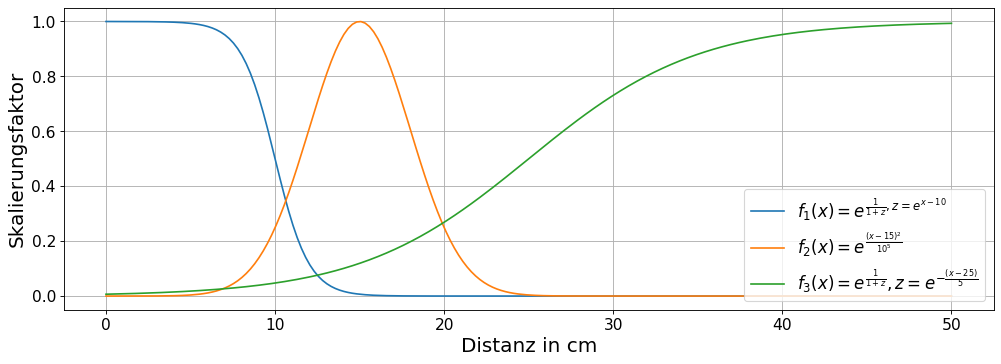
\includegraphics[width=140mm]{figures/Forschung/SkalierungAbstandhalten.png} 
\end{tabular}
\caption{ Skalierungsfunktionen für die verschiedenen Richtungsvektoren \label{fig:abstandsfunktionen}}
\end{figure}

In Abbildung \ref{fig:abstandsfunktionen} sind die gewählten Abstandsfunktion zu sehen. Die Faktoren wurden experimentell mit Rücksicht auf den verwendeten Datensatz bestimmt. Ziel ist es drei unterschiedliche Zonen zu erzeugen, durch die die Richtungsvektoren aus den Gleichungen \ref{eq:U_r},\ref{eq:U_o} und \ref{eq:U_a} in Bezug auf die Distanz des dazugehörigen Agenten gewichten.


Der Richtungsvektor des Agenten $i$ setzt sich nun durch die Linearkombination aus den drei beschriebenen Vektoren zusammen:

\begin{subequations}
\begin{align}
d_i(t+\tau)  &= {[\alpha_{1} U_{a}(t+\tau) +\alpha_{2} U_{a}(t+\tau) +\alpha_{3} U_{a}(t+\tau)]}\label{eq:U_i1}\\
U_{i}(t+\tau) &= \gamma  \frac{d_i(t+\tau)}{|d_i(t+\tau)|} \label{eq:U_i2}
\end{align}
\end{subequations}

Die Variablen $\alpha_i$ in Gleichung \ref{eq:U_i1} gewichten den Einfluss der Zonen. Im vorherigen Modell wird das Verhalten über das justieren der Zonengröße gesteuert. Hier sind die Zonen nicht veränderbar, einzig durch die Parameter $\alpha_i$ ist es möglich das Verhalten zu ändern. Der Parameter $\gamma$ aus Gleichung \ref{eq:U_i2} streckt oder staucht den resultierenden Richtungsvektor und kann somit als zurückgelegter Weg betrachtet werden.

Reynolds erwähnt in seiner ursprünglichen Publikation keinen blinden Kegel sowie keine Richtungsbeschränkung. Für dieses Modell wird dies ebenfalls der Fall sein. Das hat zum einen Einfluss auf die Performance und zum anderen gibt es den Agenten einen größeren Freiraum, sich zu bewegen.
Nachteil ist hierbei, dass es zu unnatürlichen Bewegungsmustern kommen kann. Beispielsweise könnte ein Agent in einem nächsten Zeitschritt die entgegengesetzte Richtung einnehmen. Dies ist allerdings nur der Fall, wenn nur der Agent in unmittelbarer Laufrichtung Einfluss nimmt.

Ein wichtiger Unterschied zwischen den beiden Modellen ist an dieser Stelle anzumerken. Modell aus dem Abschnitt \ref{sec:metrischesModell} kennt das Massezentrum der Agenten nicht. Das in diesem Abschnitt vorgestellte Modell jedoch kennt das Massezentrum. Zu erkunden ob diese Annahme realistisch ist, soll allerdings nicht Teil dieser Thesis sein.

